\section{Udvidet Applikationsmodel: Sekvensdiagrammer}

\subsection{Usecase 1: Start}

\begin{figure}[!h]
\centering 
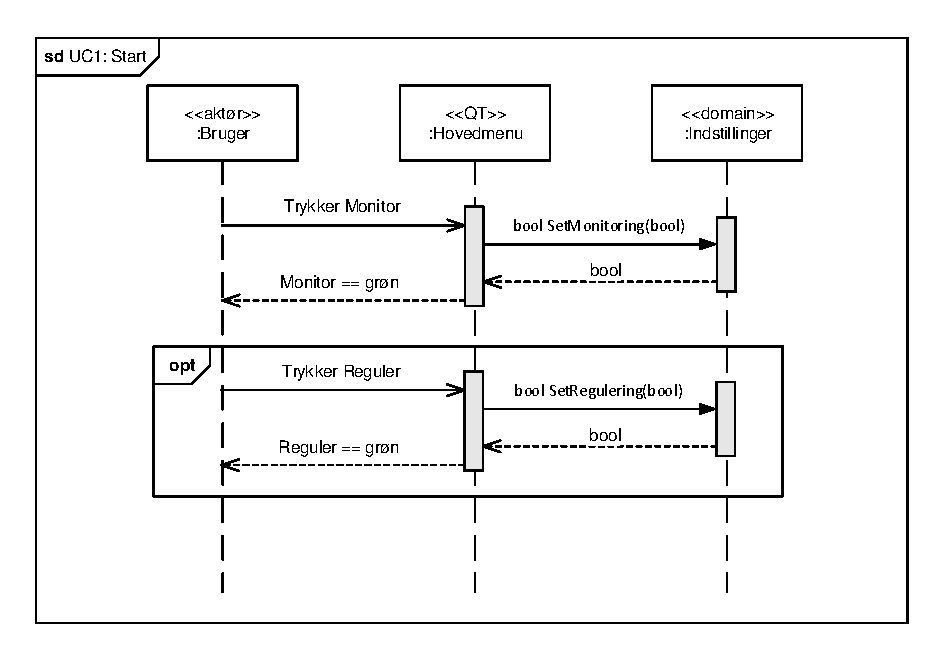
\includegraphics[width={\textwidth}, trim=0 0 0 0, clip=true] {../fig/SD_autoGreen_UC_1_Start.pdf}
\caption{Application model for UC1: Start}
\label{fig:SD_UC1}
\end{figure}

Sekvensdiagrammet for start er funktionaliten der skal forgå når der startes for monitorering, og også funktionaliteten for regulator hvis den også tændes.

\clearpage

\subsection{Usecase 2: Stop}

\begin{figure}[!h]
\centering 
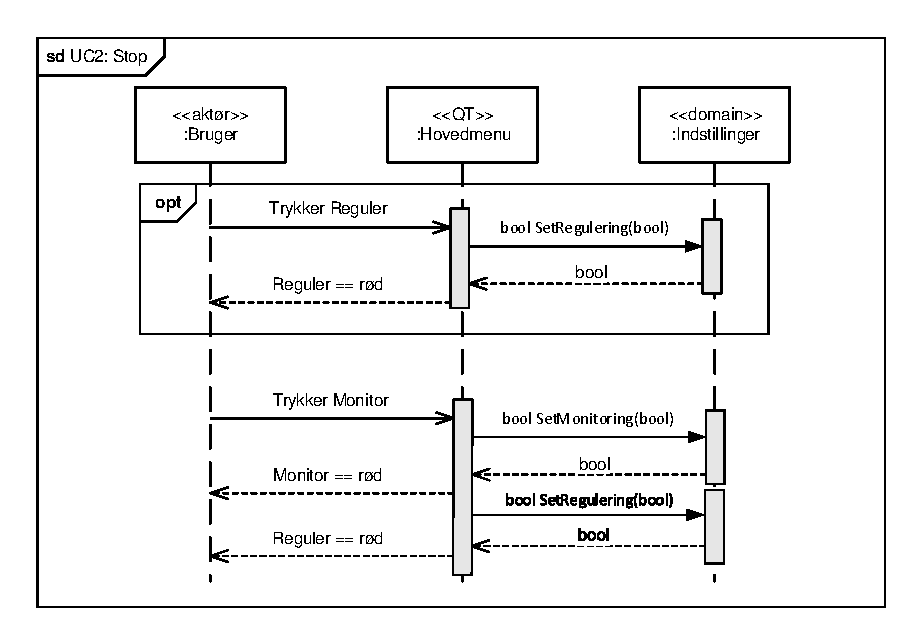
\includegraphics[width={\textwidth}, trim=0 0 0 0, clip=true] {../fig/SD_autoGreen_UC_2_Stop.pdf}
\caption{Application model for UC2: Stop}
\label{fig:SD_UC2}
\end{figure}

Sekvensdiagrammet for stop, når der ønskes at stoppe for monitorering og/eller regulering. Tryk på monitorering på begge er tændt, resultere i at både regulator og monitor slukkes.

\clearpage

\subsection{Usecase 4: Administrer Drivhus}

\begin{figure}[!h]
\centering 
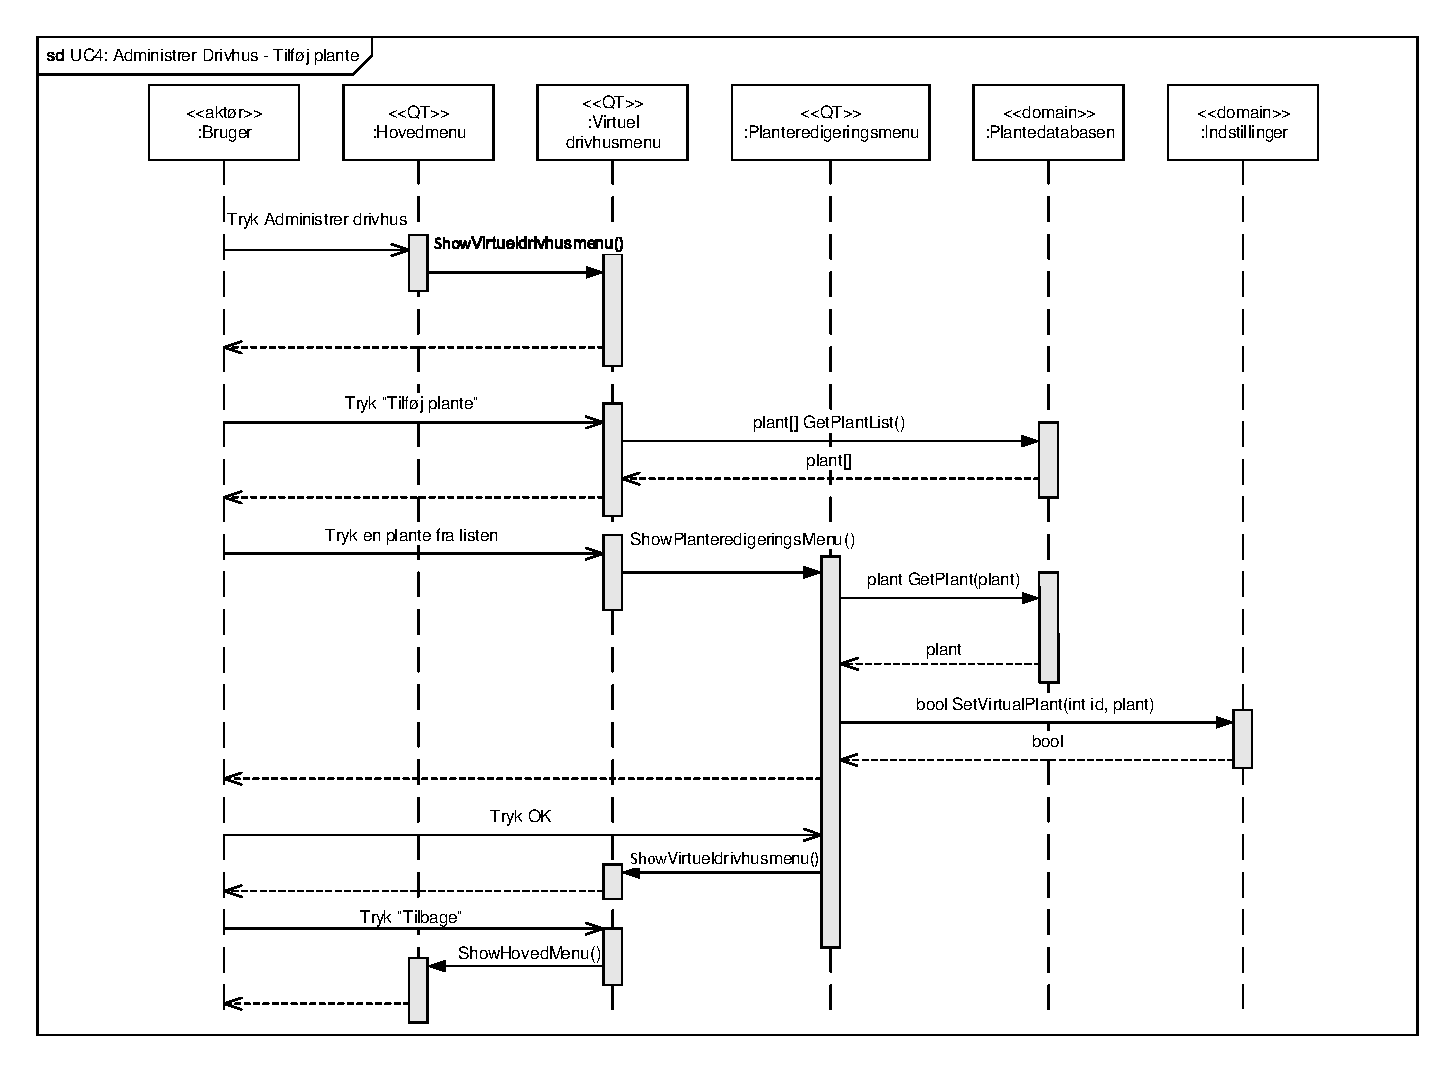
\includegraphics[width={\textwidth}, trim=0 0 0 0, clip=true] {../fig/SD_autoGreen_UC_4_Administrerdrivhus.pdf}
\caption{Application model for UC4: Administrer Drivhus - Tilføj Plante}
\label{fig:SD_UC4}
\end{figure}

Adminstre drivhus sekvensdiagrammet giver overblik over hvad der fortages når der ønskes at tilføje en plante igennem det virtuelle drivhus.

\clearpage

\begin{figure}[!h]
\centering 
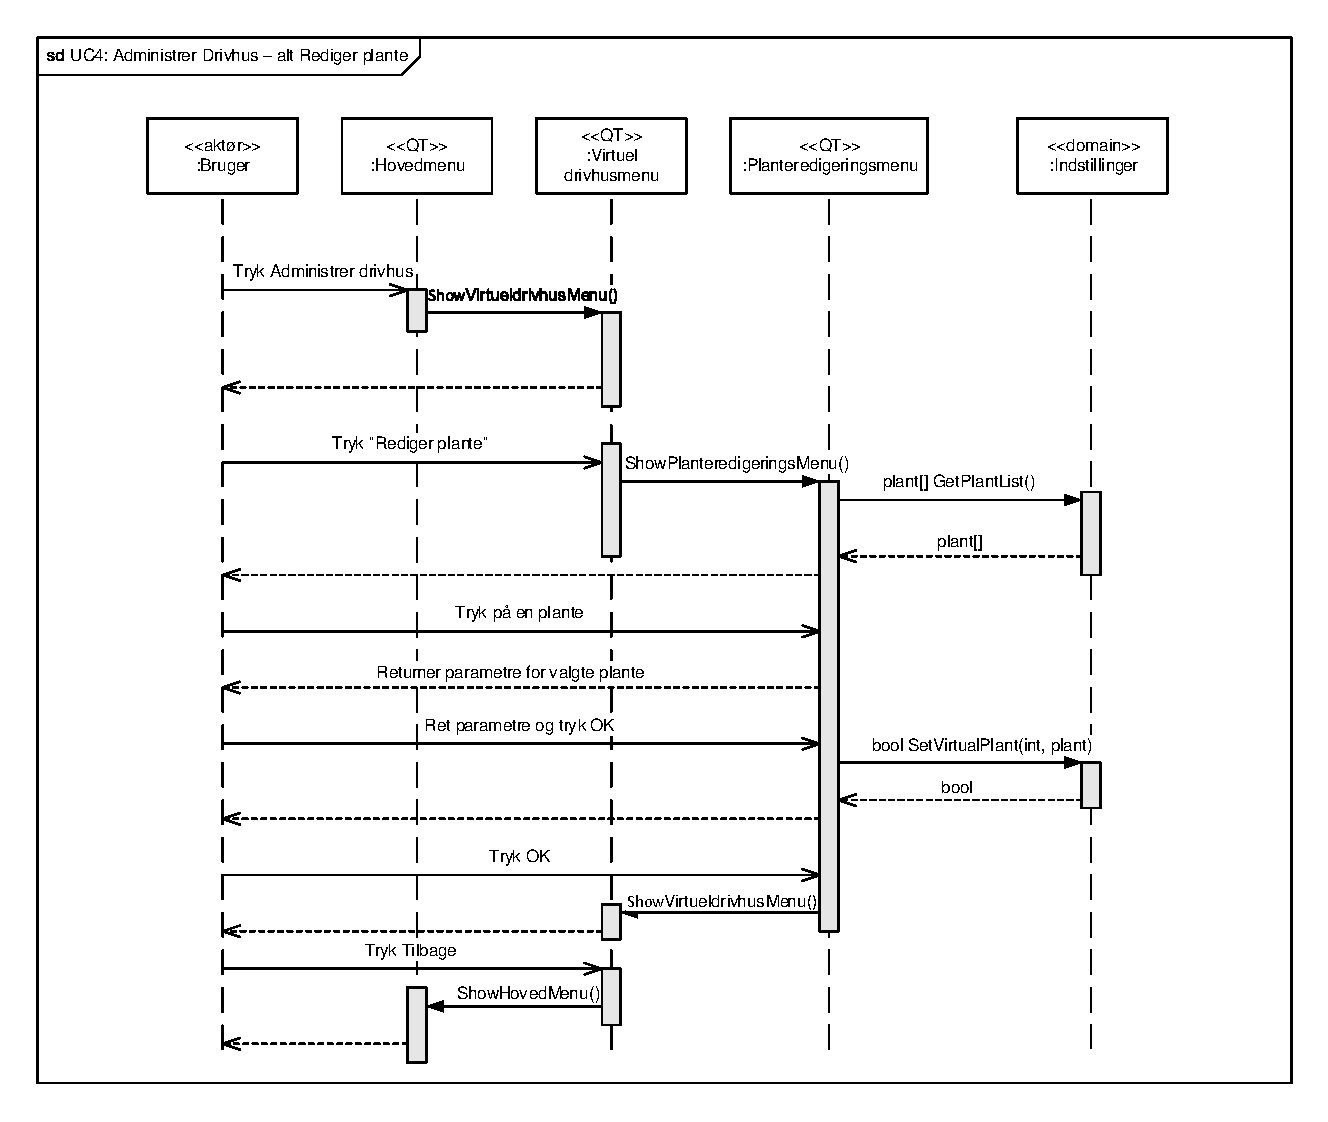
\includegraphics[width={\textwidth}, trim=0 0 0 0, clip=true] {../fig/SD_autoGreen_UC_4_Administrerdrivhus_alt_redigerplante.pdf}
\caption{Application model for UC4: Administrer Drivhus - [alt] Rediger Plante}
\label{fig:SD_UC4_alt1}
\end{figure}

Sekvensdiagrammet giver overblik over hvad der fortages i softwaren, når det ønskes at redigere en af de allerede tilstedeværende planter i det virtuelle drivhus.

\clearpage

\begin{figure}[!h]
\centering 
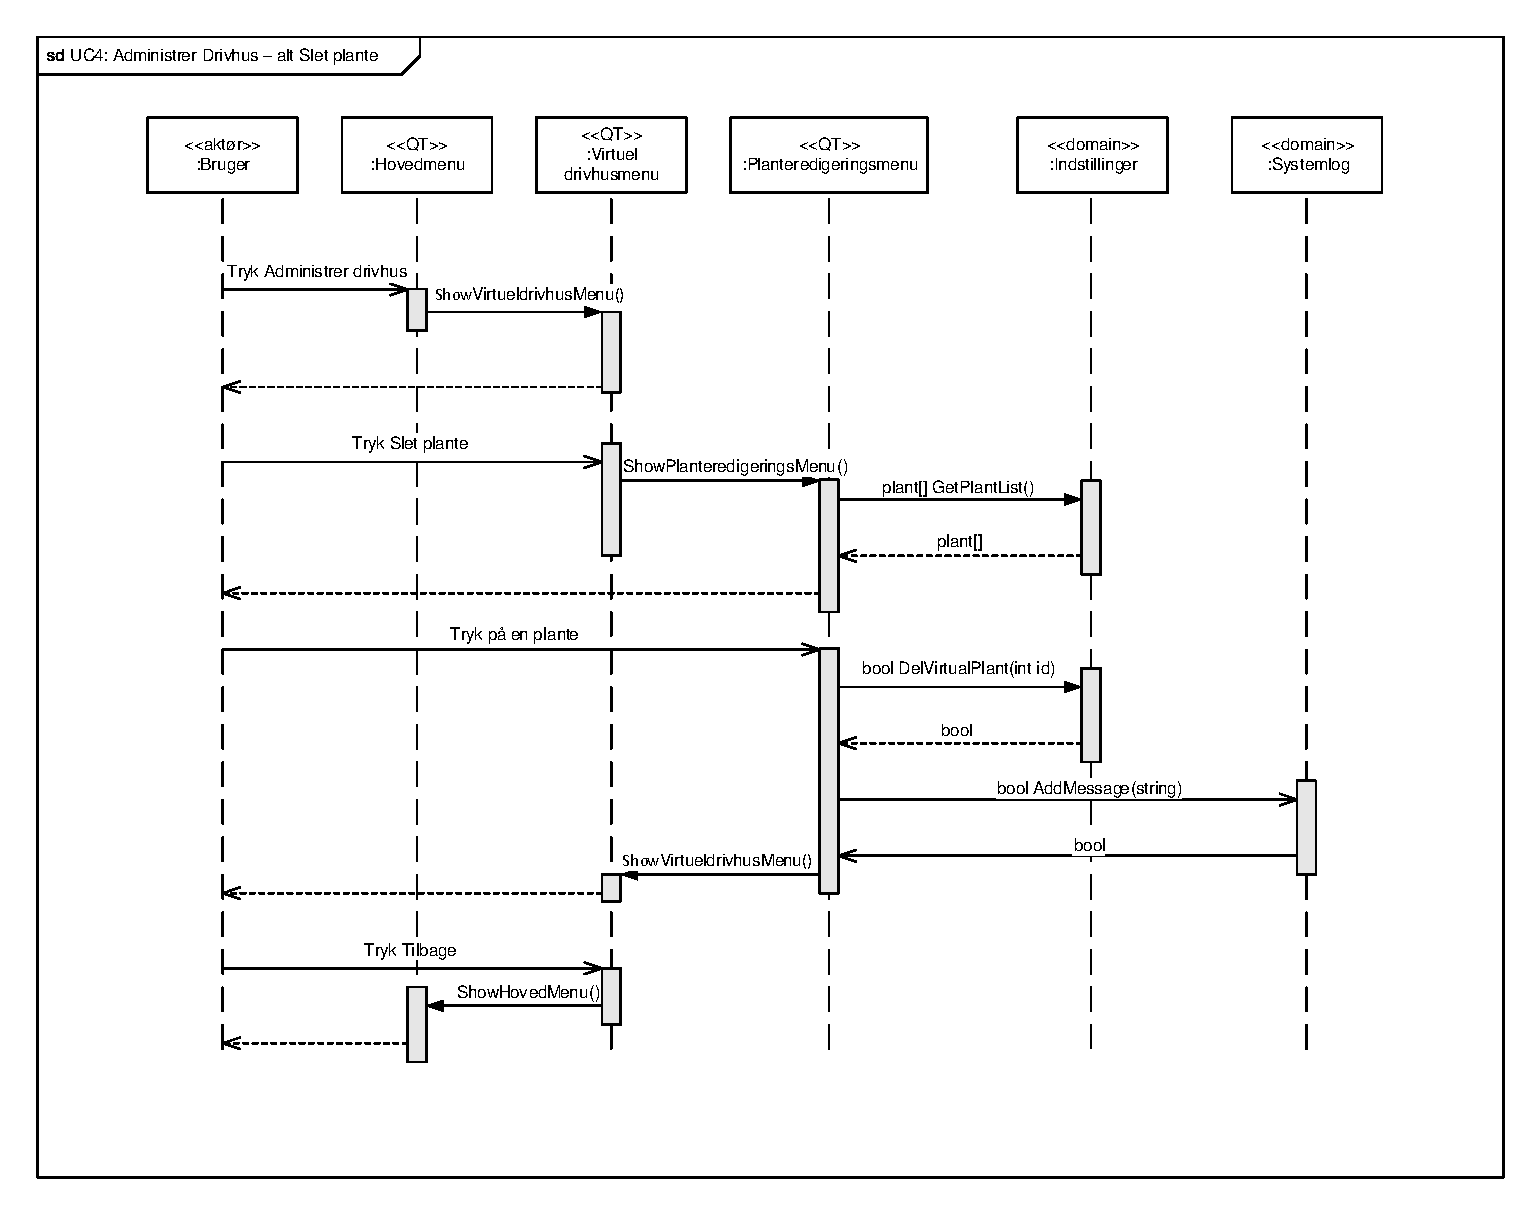
\includegraphics[width={\textwidth}, trim=0 0 0 0, clip=true] {../fig/SD_autoGreen_UC_4_Administrerdrivhus_alt_sletplante.pdf}
\caption{Application model for UC4: Administrer Drivhus - [alt] Slet Plante}
\label{fig:SD_UC4_alt2}
\end{figure}

Sekvensdiagrammet giver overblik over hvad der fortages i softwaren, når det ønskes at fjerne en tilstedeværende plante fra det virtuelle drivhus.

\clearpage

\subsection{Usecase 5: Vis Historik}

\begin{figure}[!h]
\centering 
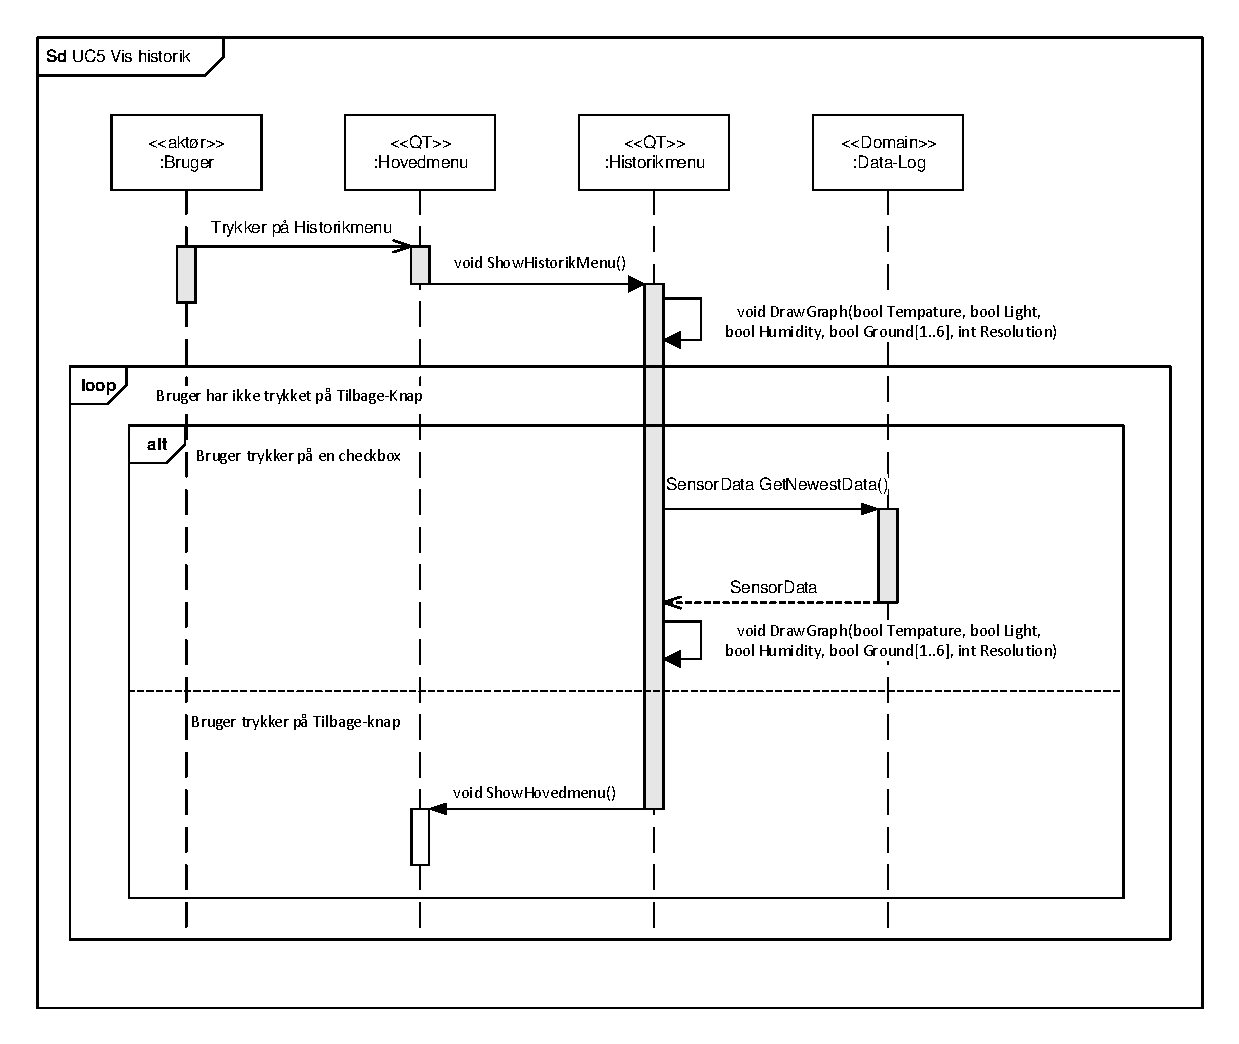
\includegraphics[width={\textwidth}, trim=0 0 0 0, clip=true] {../fig/SD_autogreen_UC_5_Vis_historik.pdf}
\caption{Application model for UC5: Vis Historik}
\label{fig:SD_UC5}
\end{figure}

Sekvensdiagrammet giver overblik over hvordan historiken fungerer, når brugeren trykker ind på 'se historik' igennem hovedmenuen.

\clearpage

\subsection{Usecase 6: Adminstrer Plantedatabase}

\begin{figure}[!h]
\centering 
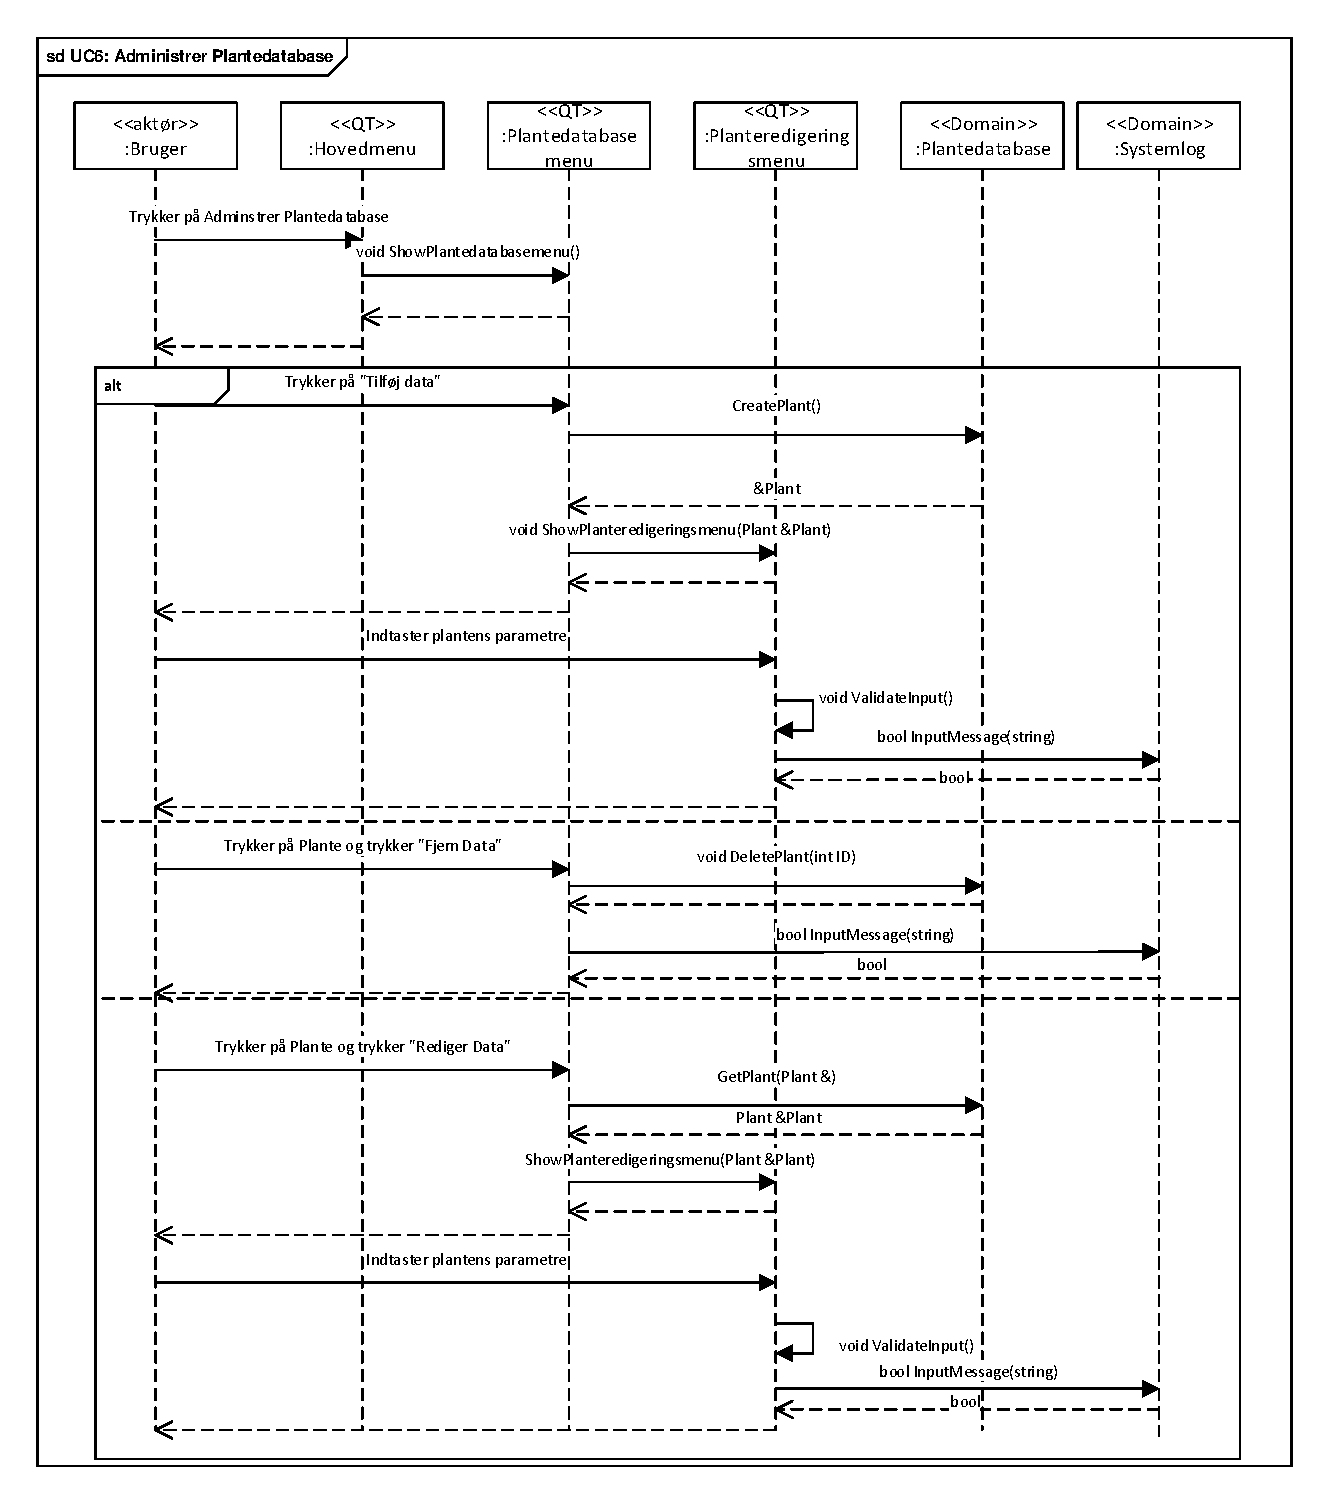
\includegraphics[width={\textwidth}, trim=0 0 0 0, clip=true] {../fig/SD_autogreen_UC_6_Adminstrer_Plantedatabase.pdf}
\caption{Application model for UC6: Administerer Plantedatabase}
\label{fig:SD_UC6}
\end{figure}

Sekvensdiagrammet giver overblik over de forskellige muligheder brugeren skal have inde fra plantedatabasen, hvorvidt en plante skal tilføjes, redigeres eller slettes.

\clearpage

\subsection{Usecase 7: Konfigurer System}

Når brugeren går ind på indstillingsmenuen bliver brugeren mødt med 4 undermenu som kan tilgåes, hertil er sekvensdiagrammerne for disse menuer.

\begin{figure}[!h]
\centering 
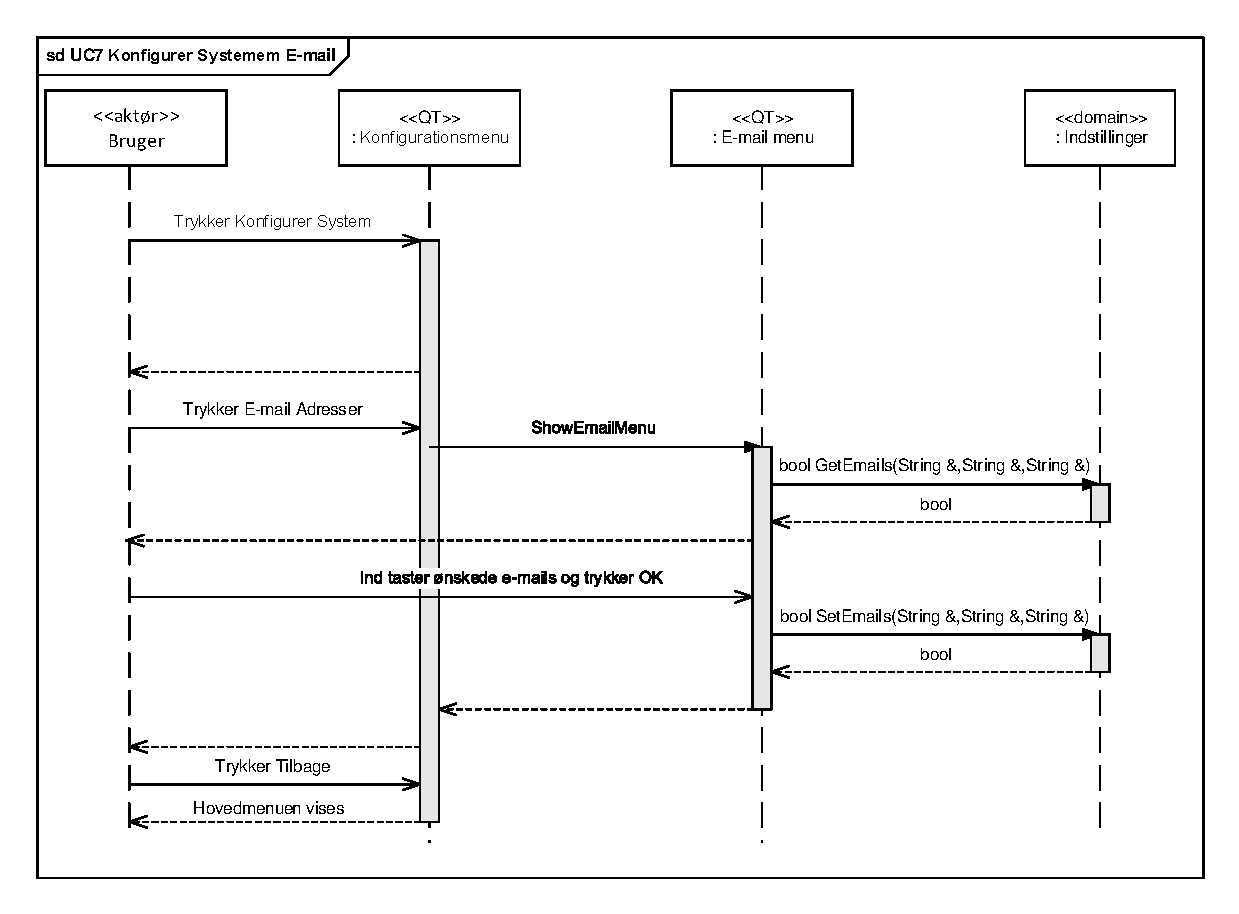
\includegraphics[width={\textwidth}, trim=0 0 0 0, clip=true] {../fig/SD_autoGreen_UC_7_E_mail.pdf}
\caption{Application model for UC7: Konfigurer System - E-mail}
\label{fig:SD_UC7}
\end{figure}

sekvensdiagrammet giver overblik over, hvordan brugeren kan skifte E-mails igennem E-mail menuen.

\clearpage

\begin{figure}[!h]
\centering 
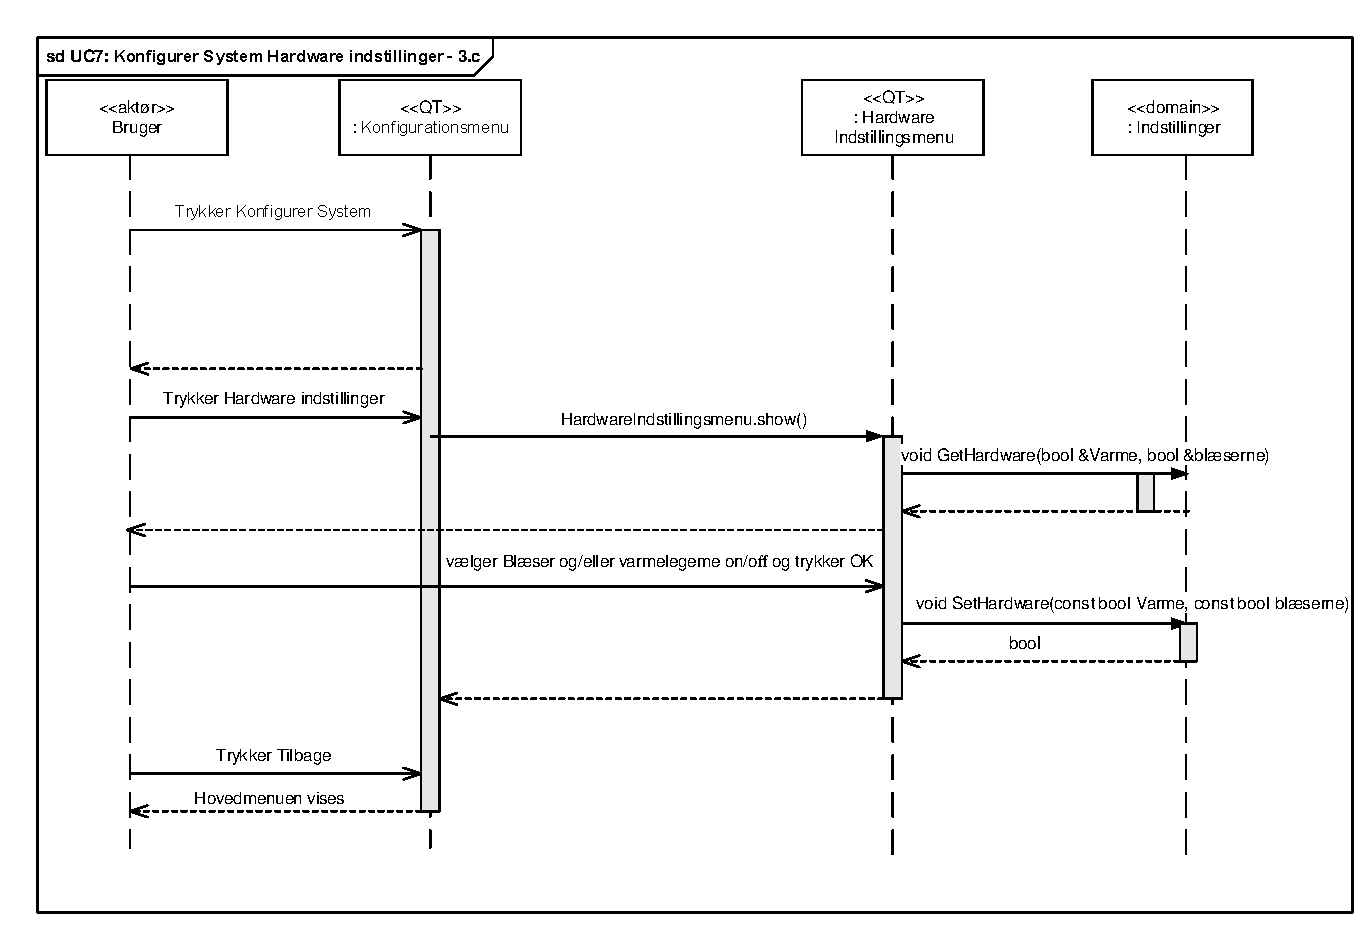
\includegraphics[width={\textwidth}, trim=0 0 0 0, clip=true] {../fig/SD_autoGreen_UC_7_Hardware_indstillinger.pdf}
\caption{Application model for UC7: Konfigurer System - Hardware Indstillinger}
\label{fig:SD_UC7_alt1}
\end{figure}

sekvensdiagrammet giver overblik over, hvordan brugeren kan skifte hardware indstillinger. Brugeren kan her vælge om blæsere og varmelegeme skal anvendes under regulering.

\clearpage

\begin{figure}[!h]
\centering 
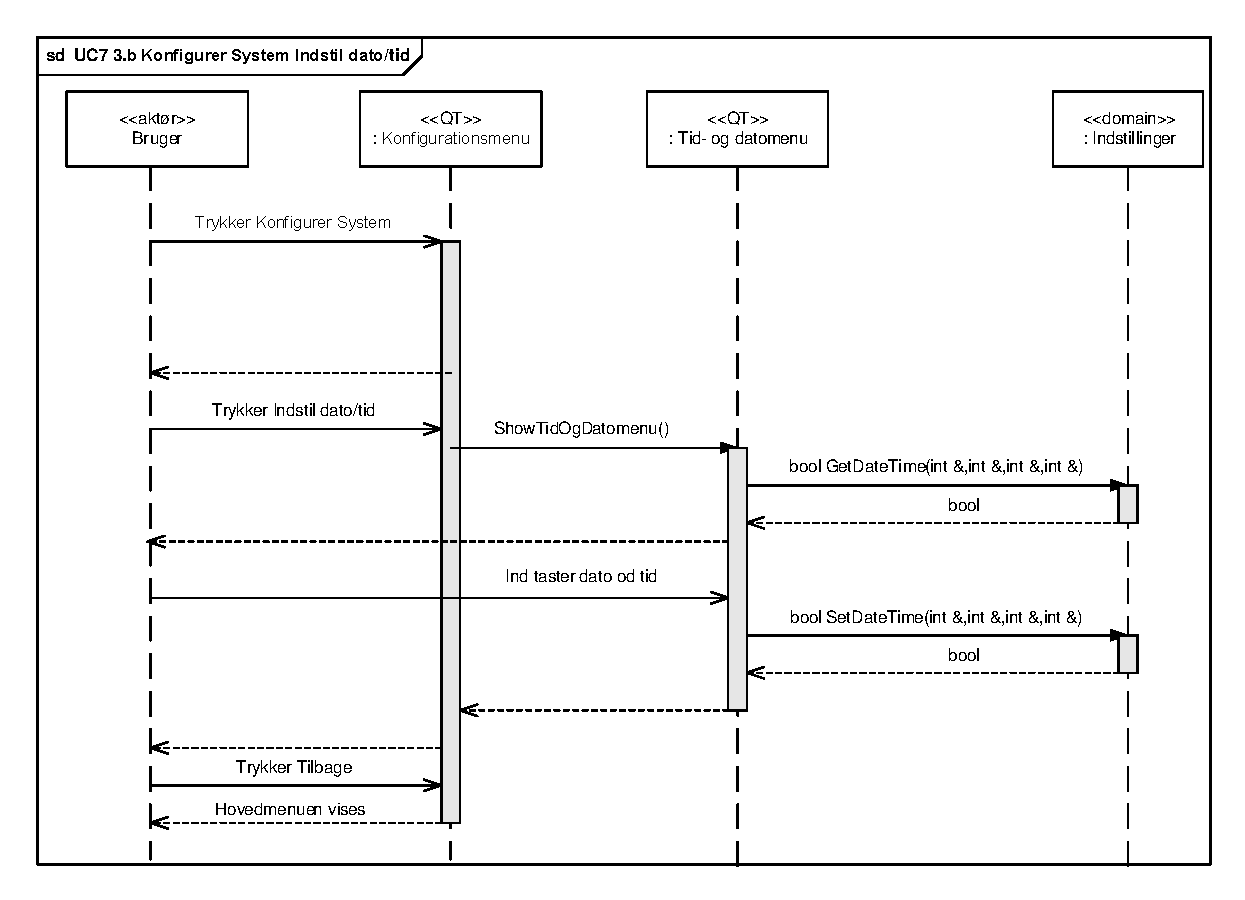
\includegraphics[width={\textwidth}, trim=0 0 0 0, clip=true] {../fig/SD_autoGreen_UC_7_Indstil_dato_tid.pdf}
\caption{Application model for UC7: Konfigurer System - Dato/Tid}
\label{fig:SD_UC7_alt2}
\end{figure}

Sekvensdiagrammet giver overblik over, hvordan brugeren kan indstille tiden på systemet.

\clearpage

\begin{figure}[!h]
\centering 
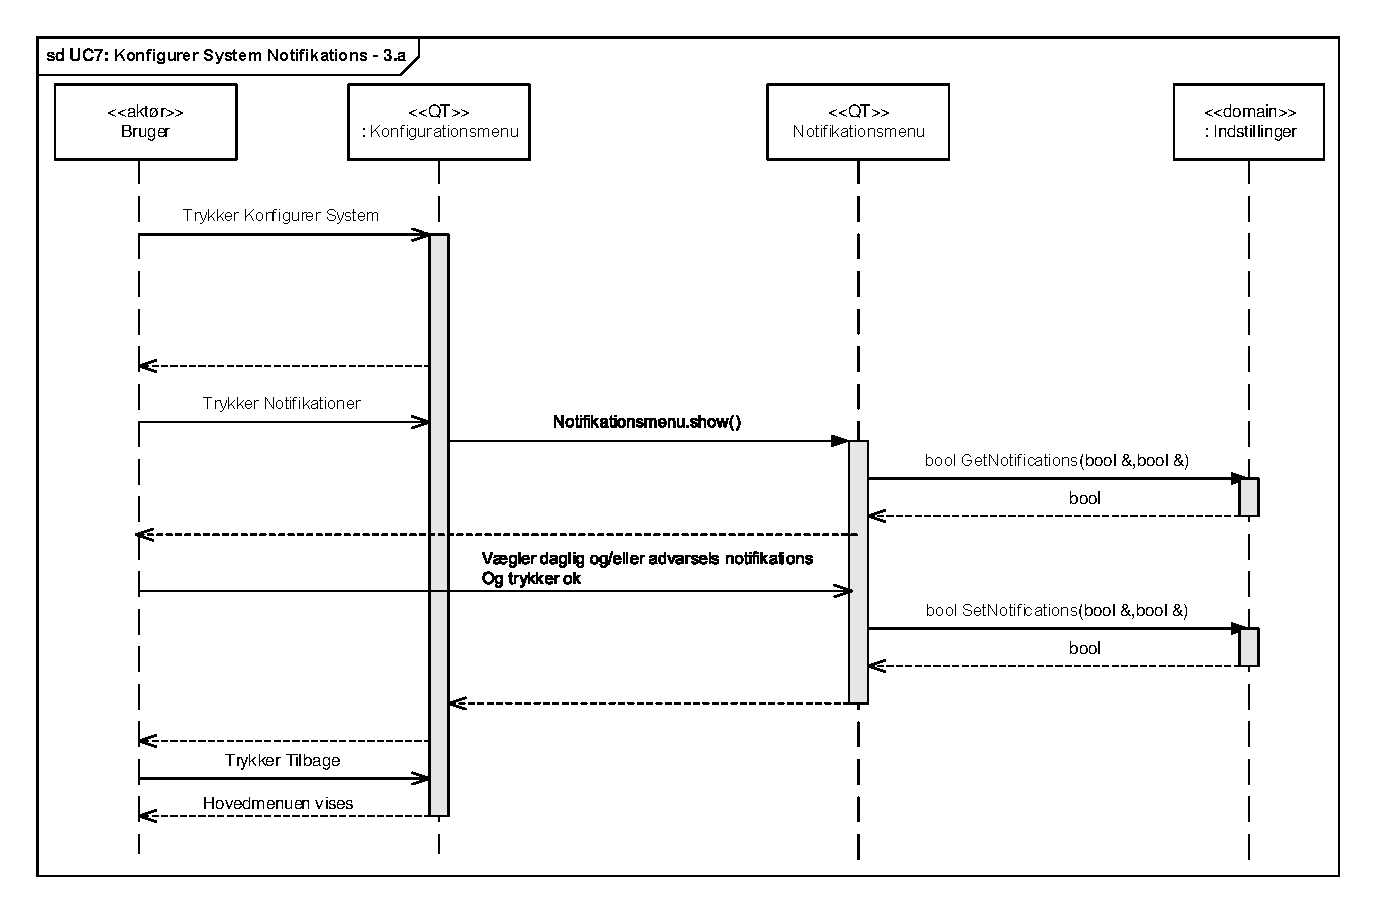
\includegraphics[width={\textwidth}, trim=0 0 0 0, clip=true] {../fig/SD_autoGreen_UC_7_Notifikationer.pdf}
\caption{Application model for UC7: Konfigurer System - Notifikation}
\label{fig:SD_UC7_alt3}
\end{figure}

Sekvensdiagrammet giver overblik over, hvordan brugeren kan aktivere og deaktivere brugen af daglige og vigtige notifikations emails fra system.

\clearpage

\subsection{Usecase 8: Se Systemlog}

\begin{figure}[!h]
\centering 
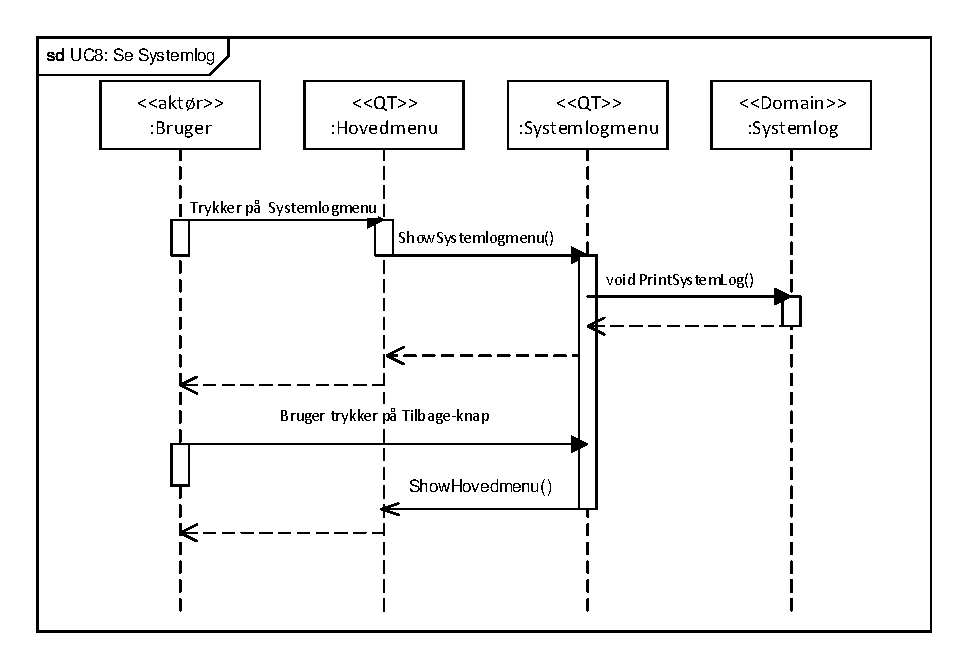
\includegraphics[width={\textwidth}, trim=0 0 0 0, clip=true] {../fig/SD_autogreen_UC_8_Se_Systemlog.pdf}
\caption{Application model for UC8: Se Systemlog}
\label{fig:SD_UC8}
\end{figure}

Sekvensdiagrammet giver overblik over hvordan brugeren kan tilgå systemloggen igennem dens egen menu. Når brugeren har tilgået menuen, udskrives de seneste systemhændelser på skærmen.

\clearpage

\subsection{Usecase 9: Rapportering}

\begin{figure}[!h]
\centering 
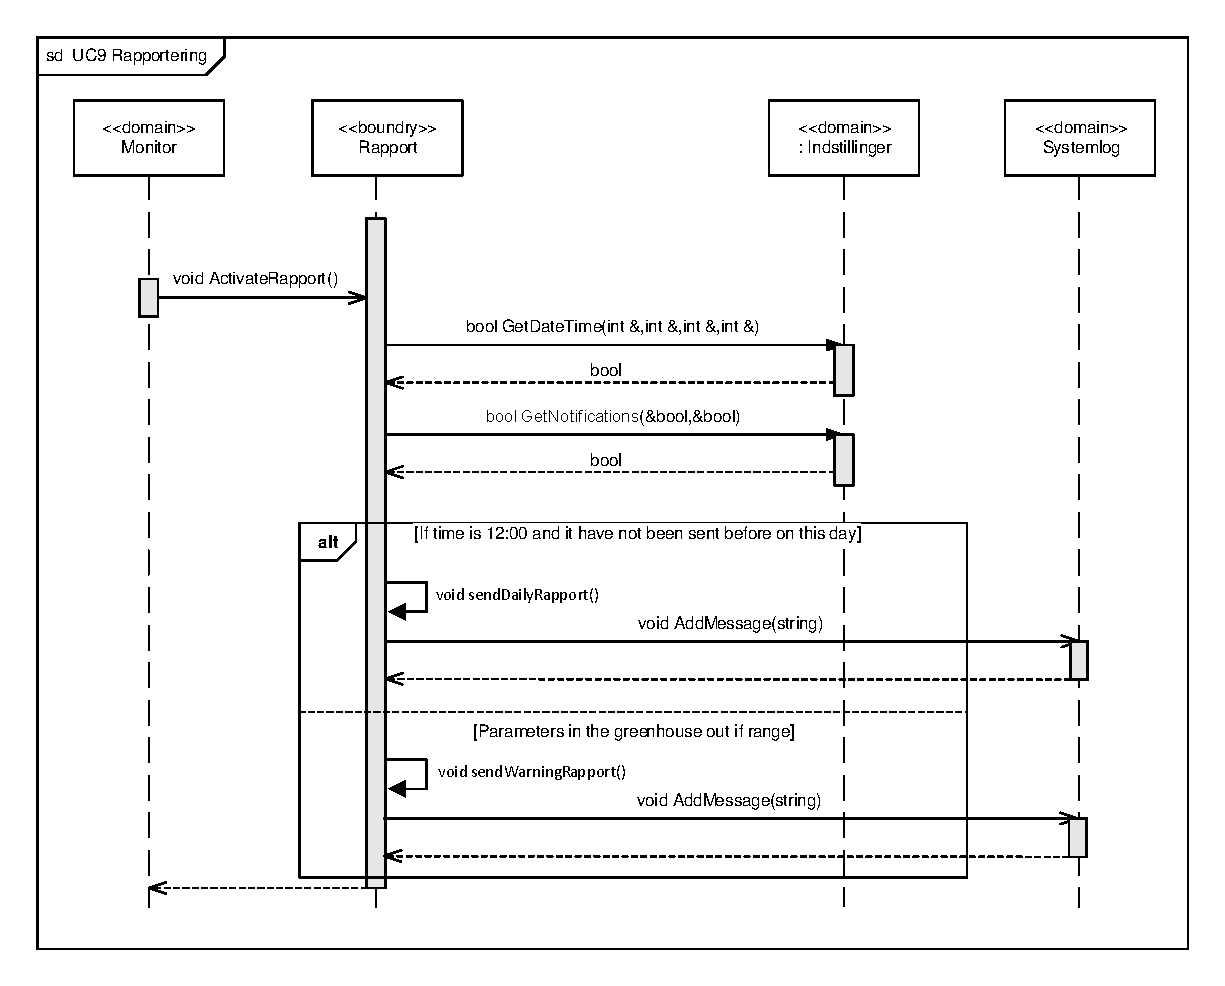
\includegraphics[width={\textwidth}, trim=0 0 0 0, clip=true] {../fig/SD_autoGreen_UC_9_Rapportering.pdf}
\caption{Application model for UC9: Rapportering}
\label{fig:SD_UC9}
\end{figure}

Sekvensdiagrammet giver overblik over, hvordan systemet kan bruger rapportering til at udsende emails til bruger, om den skal sende daglige, kun vigtige eller ingen email hentes ind fra indstillinger.

\clearpage

\subsection{Usecase 10: Monitorering}

\begin{figure}[!h]
\centering 
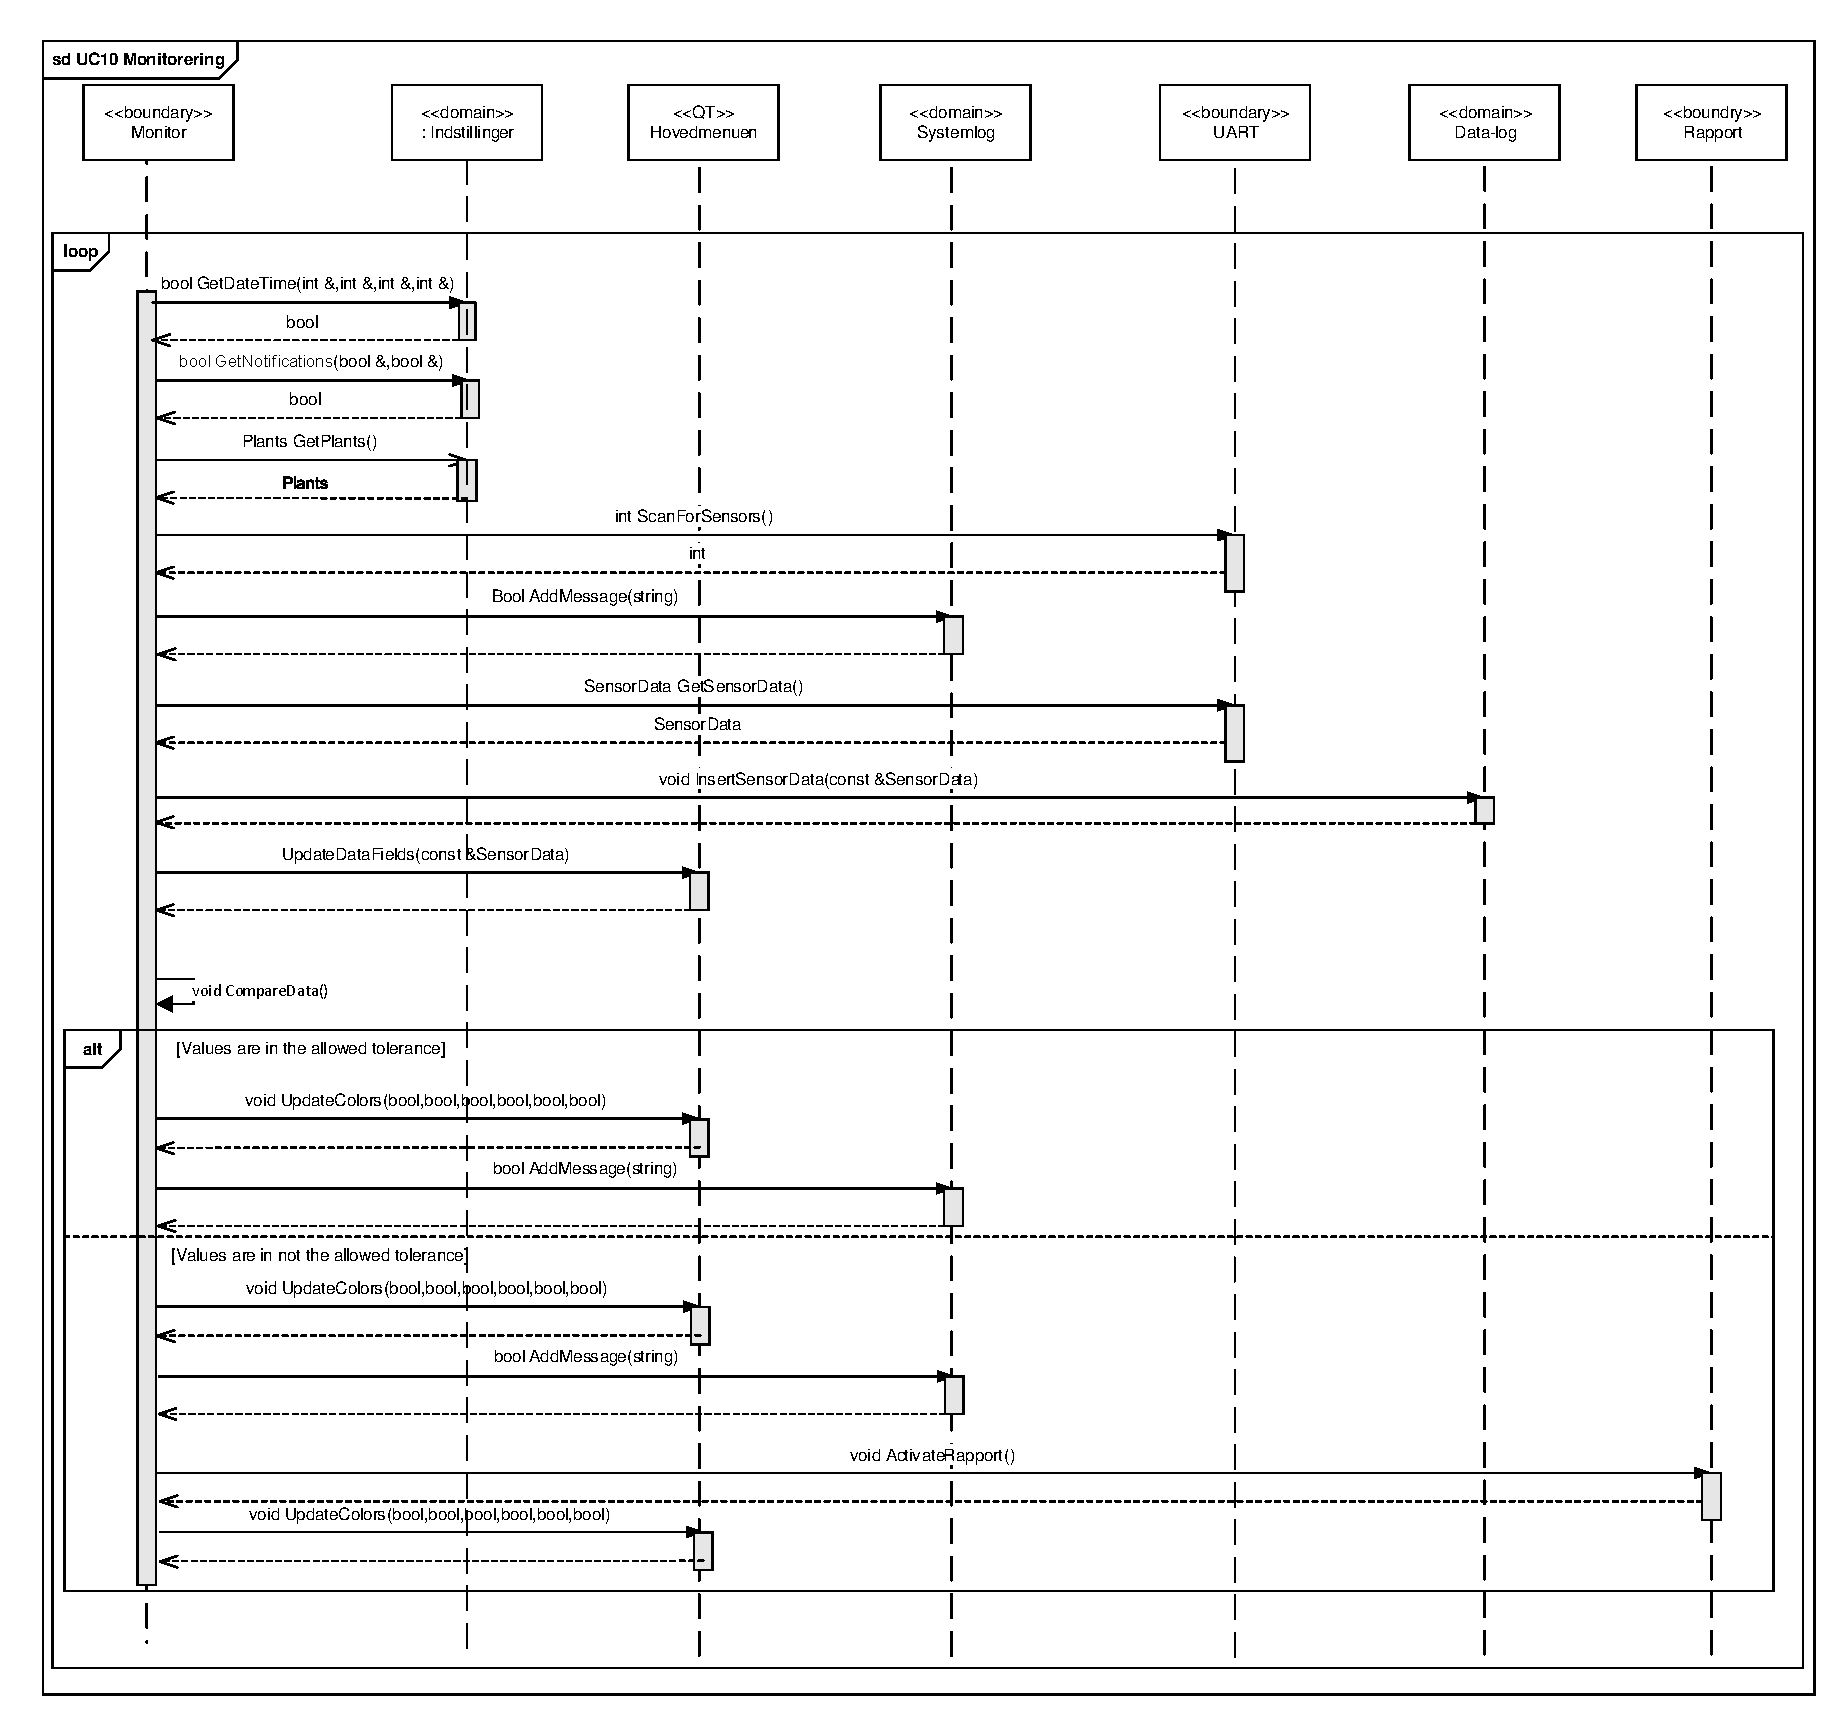
\includegraphics[width={\textwidth}, trim=0 0 0 0, clip=true] {../fig/SD_autoGreen_UC_10.pdf}
\caption{Application model for UC10: Monitorering}
\label{fig:SD_UC10}
\end{figure}

Sekvensdiagrammet giver et overblik over hvordan monitoreringstråden skal fungere, og hvilke funktionskald den skal fortage til andre klasser.

\clearpage

\subsection{Usecase 11: Regulering}

\begin{figure}[!h]
\centering 
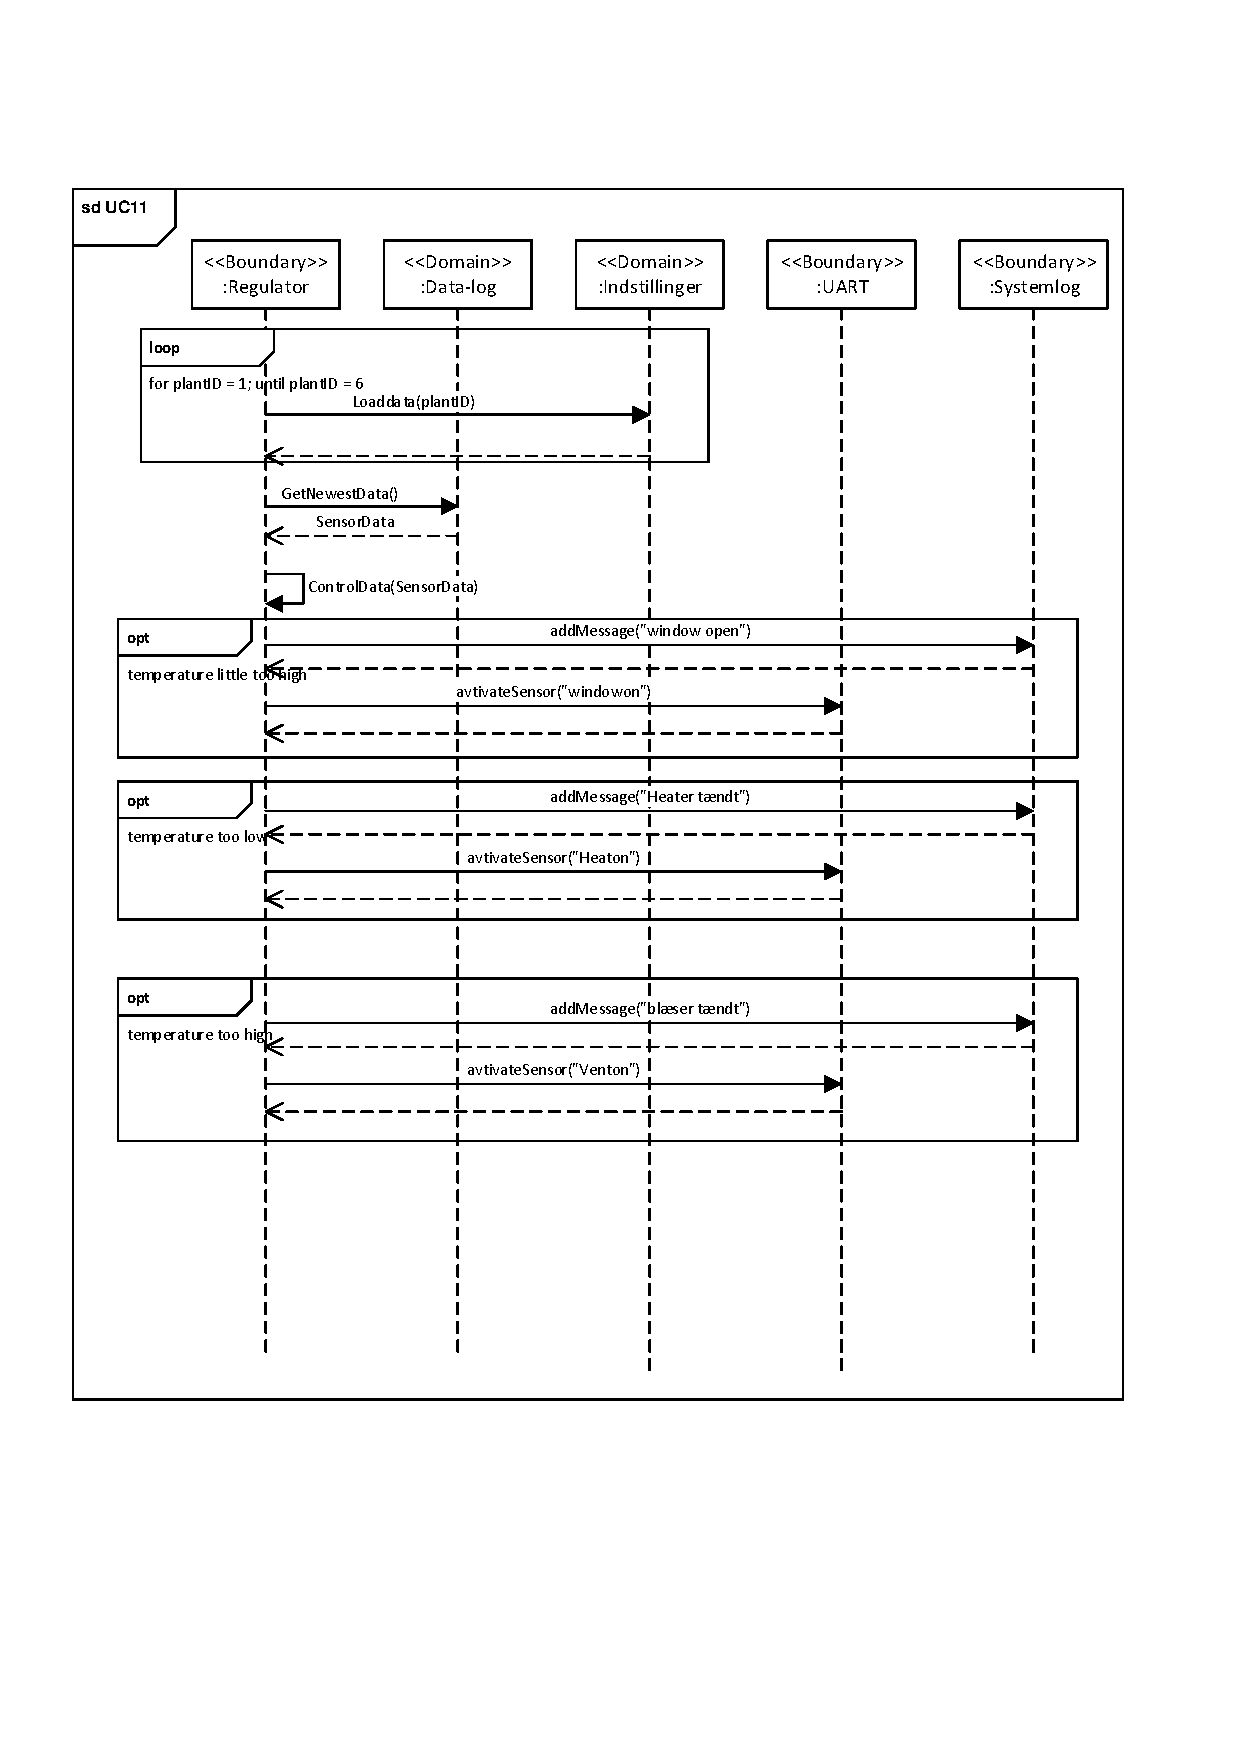
\includegraphics[width={\textwidth}, trim=0 150 0 90, clip=true]{../fig/SD_autogreen_UC_11_regulering.pdf}
\caption{Application model for UC11: Regulering}
\label{fig:SD_UC11}
\end{figure}

Sekvensdiagrammer giver overblik over hvordan reguleringstråden skal fungere, og hvilke funktionskald den skal fortage til andre klasser. f.eks. kald til UART omkring åbning eller lukning af vinduet.

\clearpage